%%%%%%%%%%%%%%%%%%%%%%%%%%%%%%%%%%%%%%%%%%%%%%%%%%%%%%%%%%%%%%%%%%%%%%%%%%%%%%%
%%                                                                           %%
%%   Dr Derek Harter                                                         %%
%%   Profesor, Department of Computer Science                                %% 
%%   Texas A&M University - Commerce, USA                                    %%
%%                                                                           %%
%%%%%%%%%%%%%%%%%%%%%%%%%%%%%%%%%%%%%%%%%%%%%%%%%%%%%%%%%%%%%%%%%%%%%%%%%%%%%%%
%%%%     SETTING STARTS - DO NOT CHANGE Unless your TeX setting require so   %%
%%%%%%%%%%%%%%%%%%%%%%%%%%%%%%%%%%%%%%%%%%%%%%%%%%%%%%%%%%%%%%%%%%%%%%%%%%%%%%%
%%----------------------------------------------------------------------------------
% DO NOT Change this. It is the required setting letterpaper page, 11pt, onside print, book style
%%----------------------------------------------------------------------------------
\documentclass[letterpaper,11pt,oneside]{book}

%%-------------------------------------
%% Page margin settings - % half inch margin all sides (recommended)
%%-------------------------------------
\usepackage[margin=1.2in]{geometry} 

%%-------------------------------------
%% Font settings - % CM San or Ariel (recommended)
%%-------------------------------------
% Switch the following two line off: to revert back to default LaTex font (NOT recommended)
\usepackage{amsfonts}
\renewcommand*\familydefault{\sfdefault}

%%-------------------------------------
%% Math/Definition/Theorem/Algorithm packages settings 
%%-------------------------------------
\usepackage[cmex10]{amsmath}
\usepackage{amssymb}
\usepackage{amsthm}
\newtheorem{mydef}{Definition}
\newtheorem{mytherm}{Theorem}

%%-------------------------------------
%% Algorithms/Code Listing environment settings  - 
%% Please do not change these settings
%%-------------------------------------
\usepackage{algorithm}
\usepackage{algpseudocode}
\renewcommand{\algorithmicrequire}{\textbf{Input:}}
\renewcommand{\algorithmicensure}{\textbf{Output:}}
\usepackage[utf8]{inputenc}
\usepackage{listings}
\usepackage{xcolor}
\definecolor{codegreen}{rgb}{0,0.6,0.1}
\definecolor{codegray}{rgb}{0.5,0.5,0.5}
\definecolor{codeblue}{rgb}{0.10,0.00,1.00}
\definecolor{codepurple}{rgb}{0.58,0,0.82}
\definecolor{backcolour}{rgb}{1.0,1.0,1.0}

\lstdefinestyle{mystyle}{
    backgroundcolor=\color{backcolour},   
    commentstyle=\color{codegreen},
    keywordstyle=\color{codeblue},
    numberstyle=\tiny\color{codegray},
    stringstyle=\color{codepurple},
    basicstyle=\ttfamily\footnotesize,
    breakatwhitespace=false,         
    breaklines=true,                 
    captionpos=b,                        
    keepspaces=true,                 
    numbers=left,                    
    numbersep=5pt,                  
    showspaces=false,                
    showstringspaces=false,
    showtabs=false,                  
    tabsize=2,
    frame=none
}
\lstset{style=mystyle}

%%-------------------------------------
%% Graphics/Figures environment settings
%%-------------------------------------
\usepackage{graphicx}
\usepackage{subfigure}
\usepackage{caption}
\usepackage{lipsum}

%%-------------------------------------
%% Table environment settings
%%-------------------------------------
\usepackage{multirow}
\usepackage{rotating}
\usepackage{makecell}
\usepackage{booktabs}
%\usepackage{longtable,booktabs}

%%-------------------------------------
%% List of Abbreviations settings
%%-------------------------------------
\usepackage{enumitem}
\newlist{abbrv}{itemize}{1}
\setlist[abbrv,1]{label=,labelwidth=1in,align=parleft,itemsep=0.1\baselineskip,leftmargin=!}

%%-------------------------------------
%% Bibliography/References settings   - Harvard Style was used in this report
%%-------------------------------------
\usepackage[hidelinks]{hyperref}
\usepackage[comma,authoryear]{natbib}
\renewcommand{\bibname}{References} % DO NOT remove or switch of 

%%-------------------------------------
%% Appendix settings     
%%-------------------------------------
\usepackage[toc]{appendix}
%%%%%%%%%%%%%%%%%%%%%%%%%%%%%%%%%%%%%%%%%%%%%%%%%%%%%%%%%%%%%%%%%%%%%%%%%%%%%%%%%%%%%%%
%%%%                     SETTING ENDS                                            %%%%%%
%%%%%%%%%%%%%%%%%%%%%%%%%%%%%%%%%%%%%%%%%%%%%%%%%%%%%%%%%%%%%%%%%%%%%%%%%%%%%%%%%%%%%%%
\begin{document}

    \captionsetup[figure]{margin=1.5cm,font=small,name={Figure},labelsep=colon}
    \captionsetup[table]{margin=1.5cm,font=small,name={Table},labelsep=colon}
    \SetLipsumDefault{1}
    
    \frontmatter
    
    \begin{titlepage}      
        \begin{center}
            
\includegraphics[width=3cm]{figures/tamuc-logo.png}\\[0.5cm]
            {\LARGE Texas A\&M University - Commerce\\[0.5cm]
            Department of Computer Science}\\[2cm]
			%{\color{blue} \rule{\textwidth}{1pt}}
			
			% -------------------------------
			% You need to edit some details here
			% -------------------------------  
            \linespread{1.2}\huge {
                %%%%%%%%%%%%%%%%%%%%%%%%%%%%
                %TODO: 1 TITLE of Your PROJECT 
                %%%%%%%%%%%%%%%%%%%%%%%%%%%%
                % chnage the following line                
               Credit Card Fraud Detection using Machine Learning Algorithms
            
            }
            \linespread{1}~\\[2cm]
			%{\color{blue} \rule{\textwidth}{1pt}}
            {\Large 
                %%%%%%%%%%%%%%%%%%%%%%%%%%%%
                %TODO: 2 YOUR NAME
                %%%%%%%%%%%%%%%%%%%%%%%%%%%%             
                % chnage the following line
                Rama Venkata Sandeep Chinta
                % change end             
            }\\[1cm] 
            

            {\large 
                %%%%%%%%%%%%%%%%%%%%%%%%%%%%
                %TODO: 3 YOUR NAME Supervisor's name(s)
                %%%%%%%%%%%%%%%%%%%%%%%%%%%%             
                % change the following line                
                \emph{Supervisor:} Derek Harter, Ph.D.}\\[1cm] % if applicable
            
    		% PLEASE DO NOT CHANGE THIS TEXT %
            \large A report submitted in partial fulfilment of the requirements of\\Texas A\&M University - Commerce for the degree of\\ Master of Science in \textit{Computer Science}\\[0.3cm] 
            \vfill
            
            
            \today % Please update this date you can use \date{April 2020} for fixed date
        \end{center}
    \end{titlepage}
    
    
    % -------------------------------------------------------------------
    % Declaration
    % -------------------------------------------------------------------
    \newpage
    \thispagestyle{empty}
    \chapter*{\Large Declaration}
    % PLEASE CHANGE THIS TEXT EXCEPT YOUR NAME%
    % -------------------------------
    %TODO: PLEASE ONLY UPDATE HERE -- PLEASE WRITE YOUR NAME %    
    % ------------------------------- 
    I,
    %%%%%%%%%%%%%%%%%%%%%%%
     Rama Venkata Sandeep Chinta, % Mandatory part
    %%%%%%%%%%%%%%%%%%%%%%%
    of the Department of Computer Science, Texas A\&M University - Commerce, confirm that this is my own work and figures, tables, equations, code snippets, artworks, and illustrations in this report are original and have not been taken from any other person's work, except where the works of others have been explicitly acknowledged, quoted, and referenced. I understand that if failing to do so will be considered a case of plagiarism. Plagiarism is a form of academic misconduct and will be penalised accordingly. \\
    
    %% Please delete as appropriate. 
    \noindent
    %%%%%%%%%%%%%%%%%%%%%%%%%%%%%%%%%%%%%%%%%%%%%%% 
    %TODO 1 Consent for example copy -  we will use 
    I give consent to a copy of my report being shared with future students as an exemplar. \\
    
    \noindent
    %%%%%%%%%%%%%%%%%%%%%%%%%%%%%%%%%%%%%%%%%%%%%%% 
    %TODO 2 Consent to let the report to use use by library for public use
    I give consent for my work to be made available more widely to members of TAMUC and public with interest in teaching, learning and research. 
    %%%%%%%%%%%%%%%%%%%%%%%%%%%%%%%%%%%%%%%%%%%%%%%
    ~\\[1cm]
    \begin{flushright}
	%------------------------------ 
	% change the following line
    %TODO: PLEASE UPDATE  Your Name  -------------------------------%
	Rama Venkata Sandeep Chinta % Please change it to your name
    
    \today
    \end{flushright}

     
    % -------------------------------------------------------------------
    % Abstract and Acknowledgement
    % -------------------------------------------------------------------
    
    %Two resources useful for abstract writing.
% Guidance of how to write an abstract/summary provided by Nature: https://cbs.umn.edu/sites/cbs.umn.edu/files/public/downloads/Annotated_Nature_abstract.pdf %https://writingcenter.gmu.edu/guides/writing-an-abstract
\chapter*{\center \Large  Abstract}
%%%%%%%%%%%%%%%%%%%%%%%%%%%%%%%%%%%%%%
% Replace all text with your text
%%%%%%%%%%%%%%%%%%%%%%%%%%%%%%%%%%%

Credit card fraud has been a major concern for all financial institutions and banking sectors and to avoid it, strict security and safety measures are required. Due to an increase in digital transactions, a need for an efficient fraud detection system is very important as a significant rise in cybecrime has been observed. The main purpose of this report is to develop an efficient fraud detection system using various machine learning models to increase the precision and effectiveness of detecting any fraud in online credit card transactions by obtaining the past details of transactions of the customers and looking for patterns to detect any suspicious activity. A credit card fraud detection dataset is used which is taken from an online source. This dataset contains all the necessary information which is required by the models to train and detect fraud easily. The first step is to clean and process the data to extract the relevant information which is then used to train the various machine learning models to detect fraud. Various machine learning models used are Logistic Regression, Decision Tree Classification, and Random forest classification which train on the processed data and are efficient in giving accurate results. These models are evaluated based on certain performance metrics like precision, F1 score, and recall and also guarantee the best possible balance between false positives and false negatives,  which can be assessed to provide the financial sectors with a more efficient approach to detect and avoid fraud activities while doing online transactions.

%%%
~\\[1cm]%REMOVE THIS



%%%%%%%%%%%%%%%%%%%%%%%%%%%%%%%%%%%%%%%%%%%%%%%%%%%%%%%%%%%%%%%%%%%%%%%%%s
~\\[1cm]
\noindent % Provide your key words
\textbf{Keywords:} Logistic Regression, Decision Tree Classification, Random forest classification, F1 Score, False Positives, False Negatives

\vfill
\noindent



    % -------------------------------------------------------------------
	% Acknowledgement
	% -------------------------------------------------------------------
   
    \chapter*{\center \Large  Acknowledgements}
%%%% Update with your text %%%%%%%%%%%%%%%
An acknowledgements section is optional. You may like to acknowledge the support and help of your supervisor(s), friends, or any other person(s), department(s), institute(s), etc. If you have been provided specific facility from department/school acknowledged so.  

   
    
    % -------------------------------------------------------------------
    % Contents, list of figures, list of tables
    % -------------------------------------------------------------------
    
    \tableofcontents
    \listoffigures
    
    \chapter*{List of Abbreviations}
\chaptermark{List of Abbreviations}
%%%%%%%%%%%%%%%%%%%%%%%%%%%%%%%%%%%
%%  Enter your list of Abbreviation and Symbols in this file
%%%%%%%%%%%%%%%%%%%%%%%%%%%%%%%%%%%
\begin{abbrv}
    
    \item[SMPCS]			School of Mathematical, Physical and Computational Sciences
    
\end{abbrv}
 %  Enter your list of Abbreviation and Symbols in this file
    
    %%%%%%%%%%%%%%%%%%%%%%%%%%%%%%%%%%%%%%%%%%%%%%%%%%%%%%%%%%%%%%%%%%%%%%%%
    %%                                                                    %%  
    %%  Main chapters and sections of your project                        %%  
    %%  Everything from here on needs updates in your own words and works %%
    %%                                                                    %%
    %%%%%%%%%%%%%%%%%%%%%%%%%%%%%%%%%%%%%%%%%%%%%%%%%%%%%%%%%%%%%%%%%%%%%%%%
    \mainmatter
    % Read for preparation of document in LaTex 
    % Lamport, L. (1986), LATEX: A Document Preparation System, Addison-Wesley.
    
    \chapter{Introduction}
\label{ch:into} % This how you label a chapter and the key (e.g., ch:into) will be used to refer this chapter ``Introduction'' later in the report. 
% the key ``ch:into'' can be used with command \ref{ch:intor} to refere this Chapter.

With the rise of digital transactions, the chances of online fraud have also increased 
significantly. Credit cards have become an integral part of financial transactions which facilitates online commerce more easily and it is also convenient for customers. However, with an increase in the use of such online transactions, there is an increase in the risk of fraud which leads to huge losses for both customers and financial institutions. Credit card fraud happens when an unidentified user makes the transaction using someone else’s card information.
Detecting such fraud manually is a very challenging task due to such a high number of transactions every moment. To deal with this cybercrime, an efficient fraud detection system \citep{Dornadula-2019} should be established which uses various machine learning algorithms and models to accurately detect the fraud. In this research, a credit card fraud detection dataset  is taken from an online source Kaggle \citep{Kaggle}  where the data is cleaned and processed to extract relevant information which can be used as training data for the machine learning models to accurately detect the fraud. Some machine learning algorithms \citep{Shah-2023} that are used are logistic regression,decision tree classification, and random forest classification which can detect fraud based on the data of past transactions and can detect fraud in real-time which is a big advantage of using machine learning algorithms. After that, these models are further tuned for provided dataset  using techniques like hyperparameter tuning \citep{Dalal-2022} , which greatly enhances the model's performance. The training data used in these models are based on various factors like location, date and time of the transaction, past transactions, etc. The performance of these combined models is then evaluated using various evaluation metrics. Deployment of such fraud detection systems ensures safer transactions by improving online security.





%%%%%%%%%%%%%%%%%%%%%%%%%%%%%%%%%%%%%%%%%%%%%%%%%%%%%%%%%%%%%%%%%%%%%%%%%%%%%%%%%%%
\section{Background}
\label{sec:into_back}

With the rise of digital transactions, the risk of credit card fraud has escalated. Current 
fraud detection systems are struggling to keep pace with evolving tactics, prompting 
the need for more efficient solutions. This study utilizes machine learning algorithms such as 
Logistic Regression and Decision Trees to craft a responsive credit card fraud 
detection system. Prioritizing real-time adaptability, the project seeks to enhance the 
security of financial transactions, contributing to the ongoing battle against credit card 
fraud.

%%%%%%%%%%%%%%%%%%%%%%%%%%%%%%%%%%%%%%%%%%%%%%%%%%%%%%%%%%%%%%%%%%%%%%%%%%%%%%%%%%%
\section{Problem statement}
\label{sec:intro_prob_art}
How can machine learning algorithms be effectively employed to enhance the specific identification and timely detection of credit card fraud, ensuring measurable improvements in accuracy, efficiency, and relevance to contemporary fraud patterns?

%%%%%%%%%%%%%%%%%%%%%%%%%%%%%%%%%%%%%%%%%%%%%%%%%%%%%%%%%%%%%%%%%%%%%%%%%%%%%%%%%%%
\section{Aims and objectives}
\label{sec:intro_aims_obj}


\textbf{Aims:} The goal of this project is to use machine learning algorithms to create an effective credit card fraud detection system that will limit the scope of fraud by providing a reliable and flexible solution.




\textbf{Objectives:} First, we use machine learning methods, including Random Forest Classification, Decision Tree Classification, and Logistic Regression, to analyse historical credit card transaction data. The focus is on training the models to recognise anomalies in transaction behaviour and spotting patterns suggestive of fraudulent activity. Second, the research seeks to implement and assess the developed models in a real-time context, ensuring the system's capability to swiftly detect and mitigate potential fraud during 
live transactions. Additionally, the study aims to contribute to the existing knowledge in credit card fraud detection by evaluating and comparing the effectiveness of various 
machine learning approaches.



%%%%%%%%%%%%%%%%%%%%%%%%%%%%%%%%%%%%%%%%%%%%%%%%%%%%%%%%%%%%%%%%%%%%%%%%%%%%%%%%%%%
\section{Solution approach}
\label{sec:intro_sol} % label of Org section
In this research work, several models are merged to produce more relevant and effective results. A grid-based searching technique is then implemented and two classifiers—a tree-based model and a liner-based model—are integrated from a variety of models, including Support Vector Machine (SVM), K-means Classification, Decision Tree classifiers, and Regression-based classifiers using the training data set provided to the model as an input which is the processed data. These models are then optimized using methods like hyperparameter tweaking for the given dataset, which significantly improves the model's performance in an optimal way. However, determining the best set of hyperparameters may be difficult and time-consuming, particularly when dealing with a wide variety of hyperparameters and intricate models like LightGBM and XGBoost. The training of the trees by gradient boost technique is optimized by the use of XG Boost which is an Extreme Gradient Boosting algorithm. It is monitored and incredibly adaptable and effective. Large data sets may be utilized for regression and classification and it has an ease of managing the missing values very well by the use of regularization techniques L1 and L2. Improvements have been demonstrated in these areas: accuracy, sensitivity, and precision by evaluating the model on certain performance metrics like recall or precision scores, F1 measures, false negatives and false positives, etc

\subsection{A subsection 1}
\label{sec:intro_some_sub1}
You may or may not need subsections here. Depending on your project's needs, add two or more subsection(s). A section takes at least two subsections. 

\subsection{A subsection 2}
\label{sec:intro_some_sub2}
Depending on your project's needs, add more section(s) and subsection(s).

\subsubsection{A subsection 1 of a subsection}
\label{sec:intro_some_subsub1}
The command \textbackslash subsubsection\{\} creates a paragraph heading in \LaTeX.

\subsubsection{A subsection 2 of a subsection}
\label{sec:intro_some_subsub2}
Write your text here...

%%%%%%%%%%%%%%%%%%%%%%%%%%%%%%%%%%%%%%%%%%%%%%%%%%%%%%%%%%%%%%%%%%%%%%%%%%%%%%%%%%%
\section{Summary of contributions and achievements} %  use this section 
\label{sec:intro_sum_results} % label of summary of results
Describe clearly what you have done/created/achieved and what the major results and their implications are. 


%%%%%%%%%%%%%%%%%%%%%%%%%%%%%%%%%%%%%%%%%%%%%%%%%%%%%%%%%%%%%%%%%%%%%%%%%%%%%%%%%%%


    \chapter{Literature Review}
\label{ch:lit_rev} %Label of the chapter lit rev. The key ``ch:lit_rev'' can be used with command \ref{ch:lit_rev} to refer this Chapter.

Credit card fraud causes significant financial losses for both people and businesses. This can have a detrimental effect on one's physical and emotional well-being. Furthermore, the aggregate impact of credit card theft raises interest rates and expenses for all clients as these financial institutions try to offset the losses caused by fraudulent activity. Generally speaking, credit card fraud has a lot of bad effects, which emphasizes the need for ongoing efforts to strengthen cybersecurity defenses and protect individuals and businesses from such monetary loss. Credit card fraud is extremely difficult to detect and has been more common recently. This
is because credit card information, such as the credit card number and expiration date, may be used by anybody to make transactions on websites without the owner's permission. First of all, victims occasionally find that opposing such illegal activity, navigating bureaucracy, and trying to retrieve their compromised money accounts are extremely taxing and frustrating procedures. By automatically learning the transaction data represented in a hierarchical manner, these deep
learning architectures have proven to perform better than other approaches, allowing them to identify complex patterns that may be missed by traditional techniques. In order to compare alternative approaches and improve model accuracy, the primary goal of this research is to evaluate the effectiveness of the user's fraud detection model using a variety of supervised machine algorithms, deep learning models, and artificial neural networks. An effective way to improve the working and enhance the performance of the implemented models is to evaluate
and analyze the model based on various evaluation metrics and performance metrics like F1 score, False positive and False negative, precision, recall, and many more.

In addition to securing bank and credit card profits and job security, these technologies will prevent fraud from costing financial institutions billions of dollars each year. Researchers have
also looked at integrating cutting-edge methods like reinforcement learning and natural
language processing (NLP) to further enhance fraud detection systems. NLP-based techniques
use textual data, including relevant information about the cardholder like the cardholder’s name,
past transactions, and the date and time of the transaction to determine useful characteristics
for fraud detection, while reinforcement learning algorithms are constantly optimizing their fraud
detection tactics in response to environmental input. Additionally, by finding relevant features
and lowering dimensional aspects, feature engineering, and selection strategies are important in
enhancing the different capabilities of various fraud detection systems. The importance of data pretreatment techniques like normalization, outlier identification, and imputations has also been
highlighted by researchers as a way to improve the accuracy and dependability of the dataset that has been provided to the machine learning model as an input.

\section{Existing System}

Credit card fraud detection systems are very significant in the field of research of academics
and economics. Several financial and other related institutions are willing to spend large
amounts of money in order to develop an efficient system to secure the process of online
transactions using credit cards for customers. Many different researchers from all around the
world have developed various systems using different machine learning techniques to identify
and prevent online financial fraud which is increasing every day and which can impose great
losses on users and specific financial institutions. Present-day systems on credit card fraud
detection make use of various machine learning and deep learning algorithms to build artificial
neural models and different optimization techniques in order to gain the desired outcome. An
existing system \citep{Priscilla-2020} that can efficiently stop online transactions using credit cards is based on the
approach of feature selection and other different machine learning algorithms. It adopts different
boosting classifiers like the XGBoosting algorithm, light gradient boosting algorithm (LGBM),
and Classic Gradient Boosting (CatBoost) to inspect the classification performance of the
system.

% PLEAE CHANGE THE TITLE of this section
\section{Example of in-text citation of references in \LaTeX} 
% Note the use of \cite{} and \citep{}
The references in a report relate your content with the relevant sources, papers, and the works of others. To include references in a report, we \textit{cite} them in the texts. In MS-Word, EndNote, or MS-Word references, or plain text as a list can be used. Similarly, in \LaTeX, you can use the ``thebibliography'' environment, which is similar to the plain text as a list arrangement like the MS word. However, In \LaTeX, the most convenient way is to use the BibTex, which takes the references in a particular format [see references.bib file of this template] and lists them in style [APA, Harvard, etc.] as we want with the help of proper packages.    

These are the examples of how to \textit{cite} external sources, seminal works, and research papers. In \LaTeX, if you use ``\textbf{BibTex}'' you do not have to worry much since the proper use of a bibliographystyle package like ``agsm for the Harvard style'' and little rectification of the content in a BiBText source file [In this template, BibTex are stored in the ``references.bib'' file], we can conveniently generate  a reference style. 

Take a note of the commands \textbackslash cite\{\} and \textbackslash citep\{\}. The command \textbackslash cite\{\} will write like ``Author et al. (2019)'' style for Harvard, APA and Chicago style. The command \textbackslash citep\{\} will write like ``(Author et al., 2019).'' Depending on how you construct a sentence, you need to use them smartly. Check the examples of \textbf{in-text citation} of sources listed here [This template recommends the \textbf{Harvard style} of referencing.]:
\begin{itemize}
    \item \cite{lamport1994latex} has written a comprehensive guide on writing in \LaTeX ~[Example of \textbackslash cite\{\} ].
    \item If \LaTeX~is used efficiently and effectively, it helps in writing a very high-quality project report~\citep{lamport1994latex} ~[Example of \textbackslash citep\{\} ].   
    \item A detailed APA, Harvard, and Chicago referencing style guide are available in~\citep{uor_refernce_style}.
\end{itemize}

\noindent 
Example of a numbered list:
\begin{enumerate}
    \item \cite{lamport1994latex} has written a comprehensive guide on writing in \LaTeX.
    \item If \LaTeX is used efficiently and effectively, it helps in writing a very high-quality project report~\citep{lamport1994latex}.   
\end{enumerate}

% PLEAE CHANGE THE TITLE of this section
\section{Example of ``risk'' of unintentional plagiarism}
Using other sources, ideas, and material always bring with it a risk of unintentional plagiarism. 

\noindent
\textbf{\color{red}MUST}: do read the university guidelines on the definition of plagiarism as well as the guidelines on how to avoid plagiarism~\citep{uor_plagiarism}.




% A possible section of you chapter
\section{Critique of the review} % Use this section title or choose a betterone
Describe your main findings and evaluation of the literature. ~\\

% Pleae use this section
\section{Summary} 
Write a summary of this chapter~\\
% https://guides.library.bloomu.edu/litreview
    % replace all text with your own text.
% in this template few examples are mention
\chapter{Methodology}
\label{ch:method} % Label for method chapter

\section{Importing the necessary libraries}

Importing the required Python libraries used for machine learning tasks and training models is the first step in any data processing task. These libraries facilitate various functionalities like visualization process, data manipulation, data modification, statistical analysis, training and testing of various deep learning models, and other machine learning tasks. Python has various external and built-in libraries that can be imported into the Jupyter Notebook. The libraries used for credit card fraud detection systems are as follows -

\subsection{Pandas}
Pandas is a powerful Python package made for analysis and data manipulation. It makes structured data processing simple by offering data structures like DataFrames. Pandas make it easy to effectively carry out operations like data cleansing, modification, data aggregation, data visualization, and data exploration.

\subsection{Numpy}
Numpy is a free Python software package that is intended for numerical operations on data in the form of arrays and multi-dimensional arrays. It provides standard mathematical techniques for data manipulation using linear algebra and gives users a variety of tools to manage such arrays and perform statistical operations. Basic array operations made possible by NumPy include indexing, slicing, adding, multiplying, and reshaping arrays.

\subsection{Matplotlib}
Matplotlib is a  Python data visualization package that offers a wide range of data visualization tools and functions that make data reading easy. A variety of graph types, including scatterplots, pie charts, bars, and histograms are available. Furthermore, these graphs may be exported in JPEG or PNG formats

\subsection{Seaborn}
Seaborn is one the best data visualization libraries used in Python and is a higher version of Matplotlib. It facilitates various functions and methods that can operate in data frames to perform the statistical plotting of graphs like heatmaps and histograms. Various graphs provided by this library include bar charts, histograms, error charts, scatterplots, and also heat maps which are not available in Matplotlib. It also has a feature that can select the colors that can disclose the underlying patterns and trends in the data.

\subsection{Scikit-learn}
This Python library is available as open-source and is used to build various machine learning methods. To train different machine learning methods and deep learning models, such as decision trees, support vector machines (SVM), naive Bayes, and classifiers, It also provides a variety of classification, regression, clustering, supervised and unsupervised techniques. By determining the accuracy score and producing the classification report, it also aids in evaluating the trained model's correctness; nevertheless, it cannot execute neural network models.

\subsection{Xgboost}
XGBoost, also referred to as Extreme Gradient Boost is a powerful Python module in which regression and classification are commonly used tasks. Gradient boosting methods are used by XGBoost, which is well-known for its efficiency, scalability, and operational strength. To correct mistakes produced by earlier models, these algorithms successively train inadequate learners, which are usually decision trees. Performance and utilization of resources are optimized by the library through the use of distributed and concurrent computing techniques.

\section{Data Collection}
The dataset for the credit card fraud detection system is taken from an online source Kaggle. It contains details of transactions made by the credit card by the card holders that happened in 2 days. The data set consists of 31 columns which contain the results of the transformation by PCA as numerical data input. Namely V1, V2, V3….V28 are the primary components identified by PCA. Only 2 columns which are ‘Time’ and ‘Amount’ have not undergone PCA transformation. The ‘Time’ column contains the seconds passed between each transaction and the dataset’s initial transaction. The column name ‘Amount’ contains the transaction amount which may be utilized for cost-sensitive learning based on examples. The ‘Class’ column is the answer variable and has the response as 1 in the event of fraud and 0 if no fraud is identified. It is advisable to use the Area Under the Precision-Recall Curve (AUPRC) to measure the accuracy for class imbalance ratio whereas for imbalance class, accuracy by confusion matrix is meaningless.

\begin{figure}[ht]
    \centering
    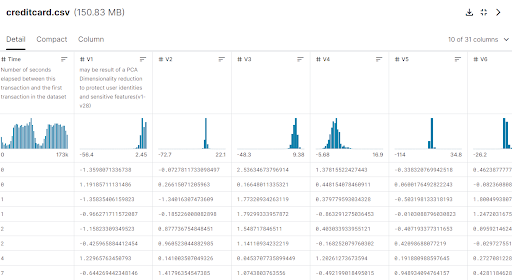
\includegraphics[scale=0.8]{figures/Data collection.png}
    \caption{Data Collection}
    \label{fig: Data Collection}
\end{figure}
.\clearpage
\section{Reading the Dataset}
Reading the Dataset is the next step after collecting the data set which is used to analyze the fraud in online transactions through credit cards. It is crucial to read the dataset after importing the required libraries to comprehend the data that has been provided. This makes it easier to train, analyze, and visualize the model of the dataset. The dataset is read by loading the CSV file into a Pandas data frame using the pd.read\_csv() function. This may be accomplished by giving the user the complete path to the CSV file or just the path to the directory in the Python environment where the dataset is uploaded. Once the dataset has been imported, data exploration is carried out. To provide an overview of the data, the top few columns and their contents are shown using the df.head() method. Here, df.head(5) provides the details of the top 5 rows and columns 


\begin{figure}[ht]
    \centering
    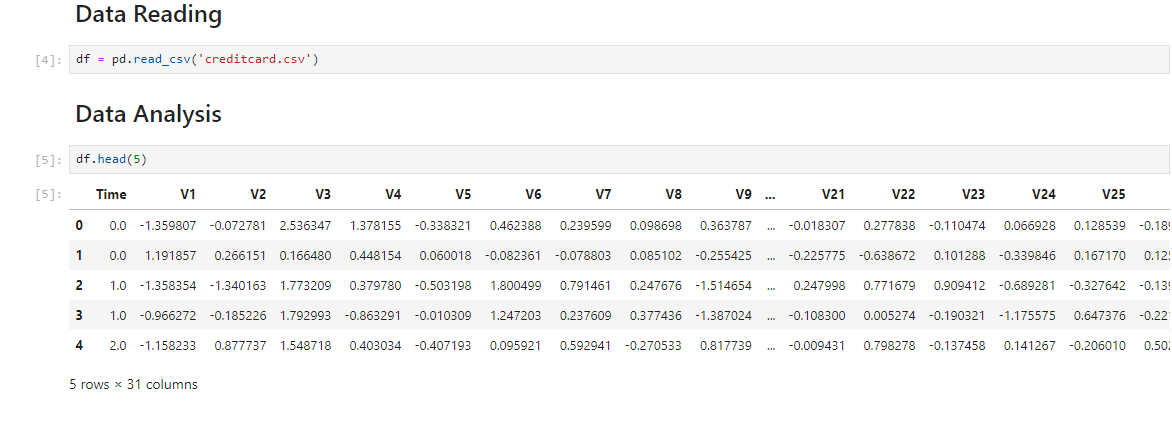
\includegraphics[scale=1]{figures/Data Reading.png}
    \caption{Fraudulent Transactions}
    \label{fig:Data Preprocessing}
\end{figure}


\section{Data Analysis}
The following step after reading the data set is to examine the substance of the data by analyzing it once the dataset has been loaded and processed in the Notebook. It entails cleansing the data by eliminating irrelevant or undesired information and handling outliers and missing numbers. After the data has been imported and cleaned, data analysis is completed. This involves examining, sanitizing, and altering the data to extract valuable insights, draw conclusions, and facilitate decision-making. Gaining understanding, making forecasts, or just working towards a particular problem's solution are all aided by data analysis. 

\begin{figure}[ht]
    \centering
    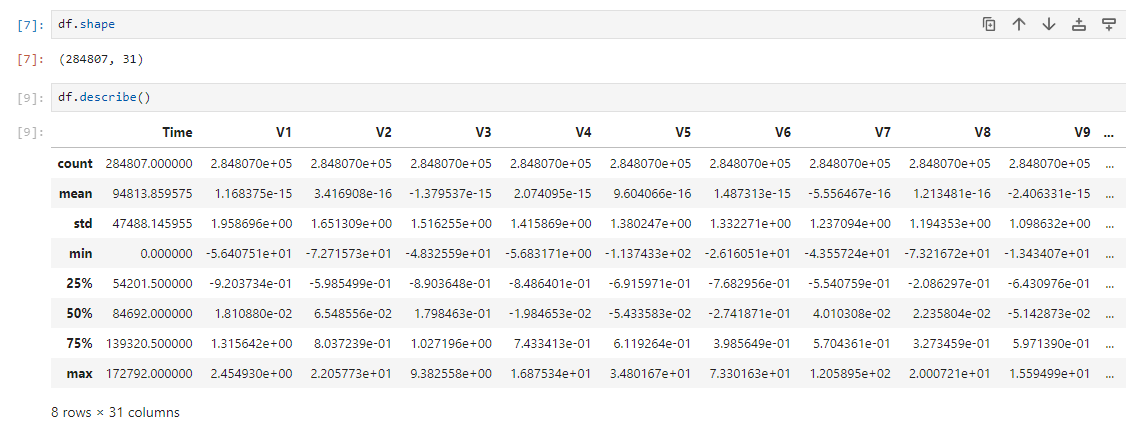
\includegraphics[scale=1]{figures/Data Analysis.png}
    \caption{Fraudulent Transactions}
    \label{fig:Data Preprocessing}
\end{figure}
\clearpage
Here, df.info() is used to get the information of the data frame which includes the data index, column name, non-null values, and the data type of that attribute. Then df.shape() is used to return the size or dimension of the data frame which is represented as the number of rows and columns. The result shows that the shape of the data frame is (284,807, 31) which denotes 284,807 rows and 31 columns. Similarly, df.describe() describes the data present in the data frame which helps to calculate statistical values like mean, median, etc. of the numerical values present in the provided data frame.


\section{Data Processing}
While processing the data set, the raw, unstructured data set is transformed into a clear, understandable form. Data pre-processing the the process of changing the data into relevant and appropriate forms before sending the data for training and testing. In this way, if the raw data contains any outliers, noise, missing values, or any irrelevant information, it can be removed before passing the data as input for the model which is the final data set. There are several  categories into which data preparation techniques are divided. Detecting outliers and addressing missing numbers are the two primary tasks of this phase. Various cleaning procedures are done to clean the data set by addressing problems which include noisy data, missing values, finding and removing outliers, and solving the differences. If users believe that the data is polluted, they are less inclined to trust data mining results. Values for a characteristic that differs from other data by more than two standard deviations might be classified as outliers. 
\begin{lstlisting}[language=Python, caption={Creating and training Catboost model}, label=list:python_code_ex]
#check if there any duplication
df.duplicated().sum()
1081

 # drop duplication data

df.drop_duplicates(inplace=True)
\end{lstlisting}

The process of data visualization is crucial to data analysis and investigation. The data visualization is supported by several built-in libraries in Python. This method presents the data in a highly graphical manner that facilitates better visual comprehension of the information, making it simpler to analyze trends and recognize patterns and correlations between several variables. Several graphs may be drawn, and each kind of graph depicts the data uniquely. The two Python libraries that are most frequently utilized when importing the graphical representation are Matplotlib and Seaborn. Many graph formats, including line, scatter, bar, and histogram plots, are supported by Matplotlib. However, Seaborn is based on Matplotlib and is an improved version of it. 

Checking for any missing values is done using the df.isna() function. Then, the data is processed for any duplicate values if present using the df.duplicates(). The result shows that there are 1081 duplicate values present in the dataset. These duplicate values are removed or dropped using the df.drop() function.

The given dataset contains the time and date of the transaction which can be used to determine the cases of fraud and valid transactions. The given data is plotted in a pie graph to visually represent the percentage of valid or legitimate transactions made with the credit card which is denoted as ‘0’ while the percentage of fraud transactions is denoted as ‘1’. The green part of the pie chart shows that ‘0’ i.e. the percentage of cases of legitimate transactions is 99.83\% while the red part of the pie chart displays the percentage of cases of fraud transactions which is 0.17\%. This data can simplify the process of identifying fraudulent transactions which helps financial institutions, and credit card owners from any fraudulent activities and transactions.


\begin{figure}[ht]
    \centering
    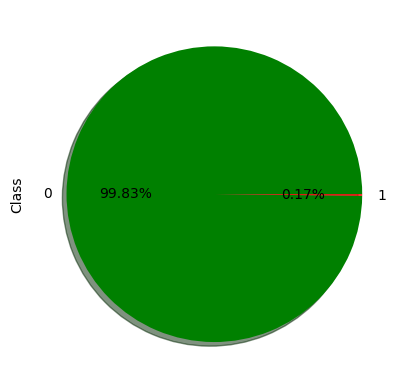
\includegraphics[scale=1]{figures/Preprocessing.png}
    \caption{Fraudulent Transactions}
    \label{fig:Data Preprocessing}
\end{figure}


\clearpage

 \section{Training and Test Split}
 After the data processing of the given dataset which includes cleaning and visualizing the data, the next step is to divide the data set into training and testing data which is used to train the deep learning model. Dividing the data set into training and testing data ensures that the model can be trained on the training part of the data and then the model can be evaluated on the testing part of the data. This can be done by using the Scikit-learn library and the data is split in such a manner that around 80\% of the data is used for the training part i.e.\textbf{ x\_train }\& \textbf{y\_train }while the remaining 20\% of the data is used for the testing i.e. \textbf{x\_test }\&\textbf{ y\_test} and evaluation part. This ensures that the data is appropriately distributed for the model to learn effectively and generate accurate predictions. Also, splitting the dataset helps to avoid overfitting issues in which the model can strongly perform on training data but poorly on new data ensuring the establishment of a robust credit card fraud detection system that works effectively in the real world.

\begin{lstlisting}[language=Python, caption={Creating and training Catboost model}, label=list:python_code_ex]
# Spliting the data into X and Y
X = df.drop(columns="Class")
y = df["Class"]

# Spliting the data into training and testing set
X_train, X_test, y_train, y_test = train_test_split(X, y, test_size=0.25, random_state=42)


# checking shape of training and testing set
print("X Train : ", X_train.shape)
print("X Test  : ", X_test.shape)
print("Y Train : ", y_train.shape)
print("Y Test  : ", y_test.shape)
\end{lstlisting}

 \section{Data Oversampling Handling}
Oversampling of data needs to be handled to increase the efficiency and quality of the sample data. One such technique to handle oversampling of data is the Synthetic Minority Over-sampling Technique (SMOTE) which is crucial to enhance the performance of the model. When the data proportion of valid transactions is comparatively larger than the fraud transaction, SMOTE helps to balance the distribution of such imbalanced data by creating data points for the minority class. In this process, new instances of the data are created using the data that is already present to improve the model’s accuracy in identifying and detecting fraud transactions.SMOTE also reduces the chance of overfitting while simultaneously increasing the size of the data set. In cases like credit card fraud detection, where even minute errors can have a huge impact or loss for the specific financial institutions. Using such an approach to handle the oversampling of data is a preventive action that strengthens the sensitivity and performance of the machine learning models that are deployed.

\begin{lstlisting}[language=Python, caption={Creating and training Catboost model}, label=list:python_code_ex]
# Apply SMOTE for solving sampling problem
smote = SMOTE(random_state=42)
X_resampled, y_resampled = smote.fit_resample(X_train, y_train)
\end{lstlisting}

 
 



\section{Implementation}
\subsection{Logistic Regression}
 Logistic Regression is a method where an outcome is determined by one or more distinct variables that may be analyzed statistically and are used to address binary classification issues and are applied in various domains like machine learning. Because of its ease of use and efficiency in forecasting the likelihood of fraudulent transactions, logistic regression can be very useful in detecting credit card fraud. Logistic Regression works by setting a specific threshold, this approach transforms the output into a probability score that falls between 0 and 1. This score can subsequently be categorized into one of two binary options: either fraud or not fraud. This method can be implemented by the Scikit-learn library by first creating the model using the \textbf{LogisticRegression()} function and then training the model with the training data x\_train and y\_train.

\begin{lstlisting}[language=Python, caption={Code snippet in \LaTeX ~and  this is a Python code example}, label=list:python_code_ex]
model = LogisticRegression()

# Training the model
model.fit(X_resampled, y_resampled)
\end{lstlisting}
 

 
After training the model, the testing set of output is predicted and the performance of the model is evaluated based on various evaluation metrics like the confusion matrix, accuracy score and the F1 score. However, the F1 Score is more reliable than the accuracy score as we are dealing with anomalies in the data which means there might be very few cases of fraud transactions out of many transactions which is a case of data imbalance. The accuracy score of the Logistic Regression model is 0.9778 and the F1 Score is 0.55075. A Confusion matrix is also plotted which shows the actual values and predicted values. 





\begin{figure}[ht]
    \centering
    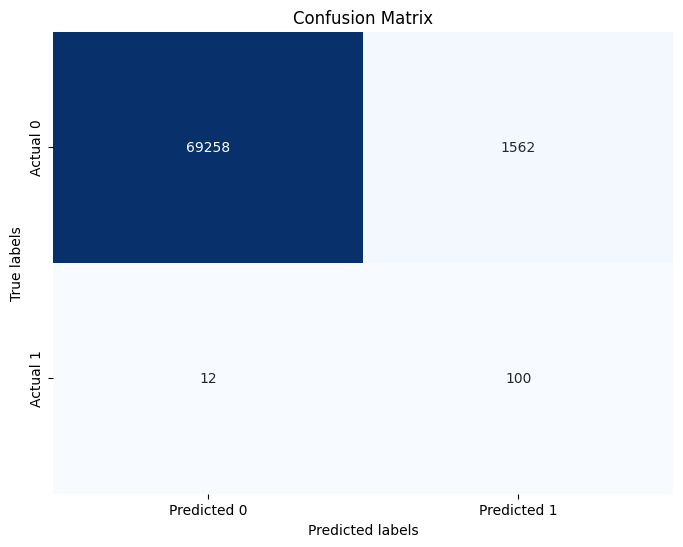
\includegraphics[scale=0.7]{figures/CM_LogisticRegression.png}
    \caption{Figure of the Data}
    \label{fig:Plot of the Data}
\end{figure}



\subsection{Grid Search Logistic Regression}

Grid search is a popular machine learning technique that goes through different values of parameters and then selects the best out of them. It is a hyperparameter tuning technique that is used to find the best parameter for a specific model. In this research, grid search is implemented along with the logistic regression model which is very essential for predicting fraud transactions in credit cards. Grid search in logistic regression is a systematic approach to assess model performance over a given grid of hyperparameters which contributes to this process by helping the logistic regression model be adjusted to achieve the ideal ratio of the difference to bias, improving the model's capacity to correctly identify fraudulent transactions. It also helps choose the best configuration by providing information on how various hyperparameters affect the performance of the model. 

\begin{lstlisting}[language=Python, caption={Code snippet in \LaTeX ~and  this is a Python code example}, label=list:python_code_ex]
# Define the logistic regression model
logistic_regression = LogisticRegression()

# Define hyperparameters to tune
param_grid = {
    'C': [0.001, 0.01, 0.1, 1, 10, 100],  # Regularization parameter
    'penalty': ['l1', 'l2']                # Penalty term
}

# Perform grid search with 5-fold cross-validation
grid_search = GridSearchCV(estimator=logistic_regression, param_grid=param_grid, cv=5, scoring='f1_macro', verbose=1)

# Fit the grid search to the data
grid_search.fit(X_resampled, y_resampled)

# Get the best parameters
best_params = grid_search.best_params_
print("Best Parameters:", best_params)

# Train the logistic regression model with the best parameters
best_model = LogisticRegression(**best_params)
best_model.fit(X_resampled, y_resampled)
\end{lstlisting}

\begin{figure}[ht]
    \centering
    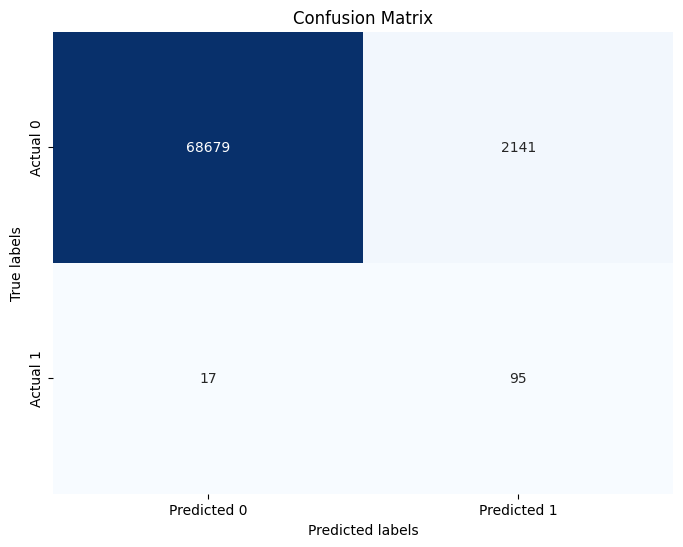
\includegraphics[scale=0.9]{figures/CM_GridSearch.png}
    \caption{Figure of the Data}
    \label{fig:Plot of the Data}
\end{figure}

\clearpage


\subsection{Random Forest Classification}

Random Forest classification is an improved version of the decision tree methodology which uses a forest made up of many trees and combines the outcome or predictions of each tree. In this forest, each tree is built using a random subset of the training dataset. This technique helps to reduce the chances of overfitting by lowering the variation of the model which is often encountered in the decision tree. The Random Forest approach produces a more accurate and dependable model when it comes to credit card fraud detection since it can handle the complicated and irregular trends in the data. The classifier is initiated by using the function \textbf{RandomForestClassifier() }and then training the classifier using the training data i.e. x\_train and y\_train. Random Forest’s ability to forecast is improved by using an ensemble approach, which allows it to recognize a wide range of fraud indications distributed over several trees. The flexibility of Random Forest to provide relevance ratings to individual features makes it a helpful  tool for identifying the primary factors influencing fraud alarms, despite its complexity and higher processing requirements compared to Decision Trees.

\begin{lstlisting}[language=Python, caption={Code snippet in \LaTeX ~and  this is a Python code example}, label=list:python_code_ex]
# Defining the Random Forest classifier
random_forest_classifier = RandomForestClassifier(n_estimators=100, random_state=42)

# Trainining the Random Forest classifier
random_forest_classifier.fit(X_resampled, y_resampled)
\end{lstlisting}


\clearpage

 After training the model, the performance of the model is evaluated based on various evaluation metrics like the confusion matrix, accuracy score and the F1 score. However, the F1 Score is more reliable than the accuracy score as we are dealing with anomalies in the data which means there might be very few cases of fraud transactions out of many transactions. The accuracy score of the Random Forest Classifier model is 0.9995 and the F1 Score is 0.9257. A Confusion matrix is also plotted which shows the actual values and predicted values.


 \begin{figure}[ht]
    \centering
    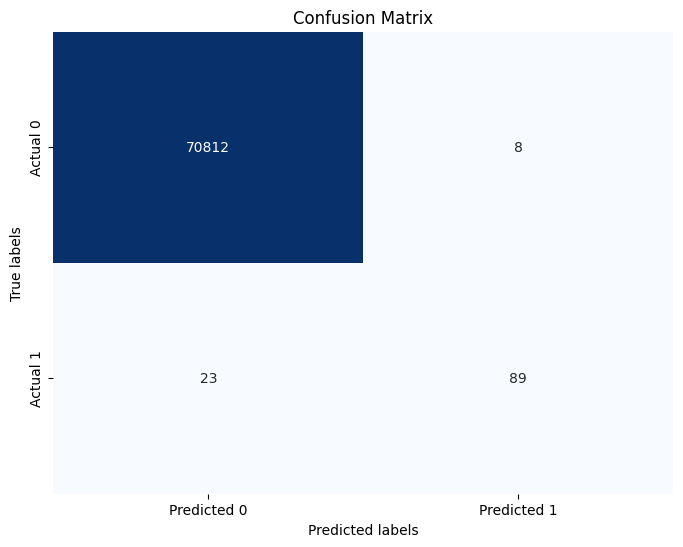
\includegraphics[scale=0.7]{figures/CM_RandomForest.png}
    \caption{Figure of the Data}
    \label{fig:Plot of the Data}
\end{figure}



 \subsection{eXtreme Gradient Boost }

 XG Boost or Extreme Gradient Boosting is a complex variant of the gradient boosting method that is recommended for its quick processing speed and outstanding effectiveness. To optimize the utilization of computing resources and raise the overall effectiveness of models, it provides a flexible and accurate method for improving decision tree models. When the number of fraud transactions is much more than the number of valid transactions, then data imbalance occurs which can be resolved by using XGBoost. To do this, it uses a gradient boosting framework, which sequentially and cautiously fixes flaws from previous models (trees). With a technique called boosting, every succeeding model seeks to gradually reduce the errors found in its earlier models.XGBoost is a helpful tool for identifying complex fraudulent behaviour in large transactional data sets due to its capacity to handle minimal data, work with a variety of loss functions, and analyze inaccurate information instantly. 
\clearpage

 \begin{lstlisting}[language=Python, caption={Code snippet in \LaTeX ~and  this is a Python code example}, label=list:python_code_ex]
# Initializing the XGBoost model
xg = xgb.XGBClassifier()

# Training the XGBoost model
xg.fit(X_resampled, y_resampled)
y_pred = xg.predict(X_test)

# Calculating AUC Curve for XGBoost
y_pred_probability = xg.predict_proba(X_test)[::,1]
fpr, tpr, _ = metrics.roc_curve(y_test, y_pred_probability)
auc = metrics.roc_auc_score(y_test, y_pred_probability)
plt.plot(fpr,tpr,label="XGBoost, auc="+str(auc))
plt.legend(loc=4)
plt.show()
\end{lstlisting}


 An important assessment indicator is the AUC (Area Under the Curve) curve generated by XGBoost in a credit card fraud detection system. This curve shows how well the model can distinguish between fraudulent and legitimate transactions across various parameters. The graph illustrates the relationship between the true positive and false positive rates, offering a significant understanding of the model's precision in detecting fraudulent transactions while mitigating false positives. When the AUC value approaches 1, it signifies that the model has a strong discriminating capacity and can effectively discriminate between fraudulent and legal transactions. The AUC score of this model is 0.9721. 

 

 A lower AUC value, on the other hand, that is closer to 0.5 denotes poorer model performance, similar to chance in class distinction. Because of this, the AUC value serves as a crucial metric for evaluating how successfully the model detects fraudulent activity while lowering false positives. It provides insightful information about the model's reliability and ability to predict outcomes in real-world situations. As the curve moves closer to the upper-left corner, indicating higher true positive rates and lower false positive rates, the model demonstrates increased filtering ability and reliability in differentiating between authentic and fraudulent behaviours. 


\begin{figure}[ht]
    \centering
    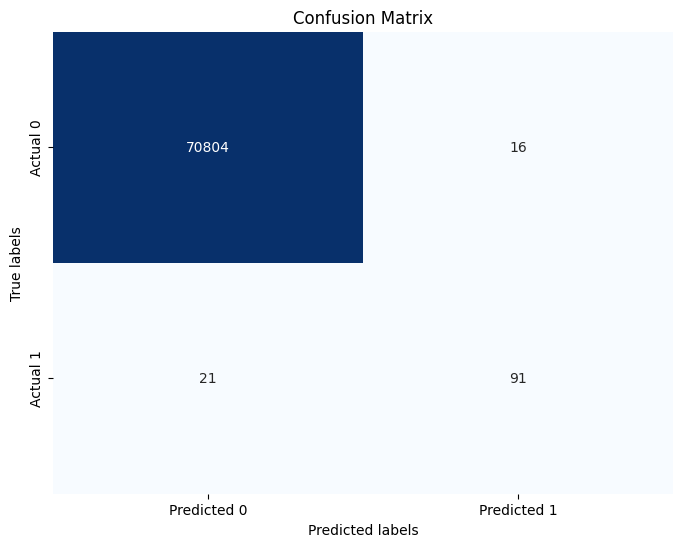
\includegraphics[scale=0.7]{figures/CM_XGBoost.png}
    \caption{Figure of the Data}
    \label{fig:Plot of the Data}
\end{figure}
 The accuracy score of the Xgboosting Classifier model is 0.9994 and the F1 Score is 0.9153 

 \begin{figure}[ht]
    \centering
    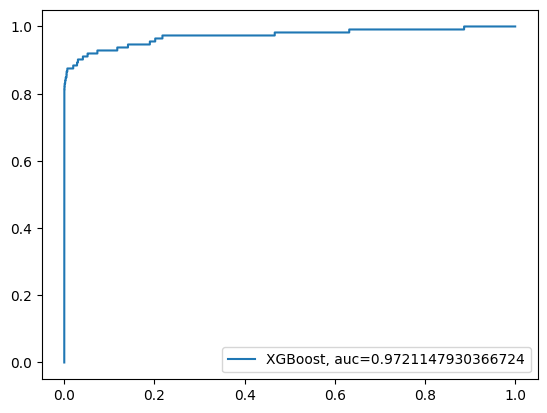
\includegraphics[scale=0.7]{figures/XGBoost.png}
    \caption{Figure of the Data}
    \label{fig:Plot of the Data}
\end{figure}

\clearpage
 \subsection{Categorical Boost}

 CatBoost, also known as Categorical Boosting is a popular machine learning approach that is built upon the gradient boosting platforms and is particularly designed to handle the categorical variables efficiently. CatBoost effectively incorporates this data to improve the recognition of fraudulent transactions in credit card fraud detection, where datasets often consist of both numerical and categorized data. CatBoost can handle the complexity of fraud detection activities with ease because of its gradient-boosting mechanism and special way of processing categorical data. This helps to prevent overfitting and maintain the highest possible accuracy. CatBoost uses a structured boosting technique to reduce the error in prediction and to provide a more accurate and reliable model. In addition, it is especially useful in complex fraud detection cases where categorization into many fraud categories is required because of its inherent capacity for multi-classification and its capacity to manage inaccurate information. Building robust and effective credit card fraud detection systems is made easier with CatBoost's versatility, ease of use, and dependability while managing a variety of data formats. The model is running for 100 iterations with a learning rate of 0.5 and the evaluation metric chosen is AUC.

 \begin{lstlisting}[language=Python, caption={Creating and training Catboost model}, label=list:python_code_ex]
# Initialize CatBoost model
cb_model = CatBoostClassifier(iterations=100,
                              depth=12,
                              eval_metric='AUC',
                              random_seed=2018,
                              od_type='Iter',
                              metric_period=1,
                              od_wait=100)

# Make predictions using the CatBoost model
cb_predict = cb_model.predict(X_test)
\end{lstlisting}
\clearpage

 The accuracy score of the Catboost Boosting Classifier model is 0.9991 and the F1 Score is 0.8769.  

\begin{figure}[ht]
    \centering
    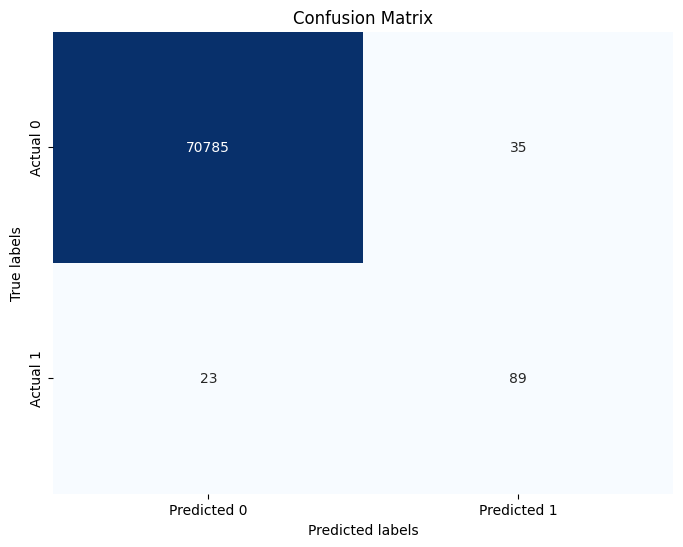
\includegraphics[scale=0.6]{figures/CM_CatBoost.png}
    \caption{Confusion Matrix}
    \label{fig:Plot of the Data}
\end{figure}

\clearpage





    \chapter{Results}
\label{ch:results}


The results obtained from the credit card fraud detection system give evidence of how well sophisticated deep learning models work for predicting unauthorized transactions. Four distinct machine-learning techniques were taught to distinguish between authentic and fraudulent transactions in this investigation. Accuracy and F1 score, which are crucial metrics for evaluating classification ability, differ throughout the models. A dataset with a variety of transactional anomalous patterns in which the models used to detect fraud transactions are Logistic Regression, Random Forest Classification, XGBoost model, and Cat Boost which can be utilized by importing the Python libraries, Scikit-learn, and xgboost. Each model is trained on the training data provided by the network and then tested against the testing data. After training these models, their performance is evaluated based on various evaluation metrics such as confusion matrix, accuracy score and F1 score. However, for this study, the F1 score is a more reliable measure to analyze the model’s efficiency than the accuracy score because of the imbalance in data as there are a large number of valid transactions and very few fraud transactions. 



 \begin{figure}[ht]
    \centering
    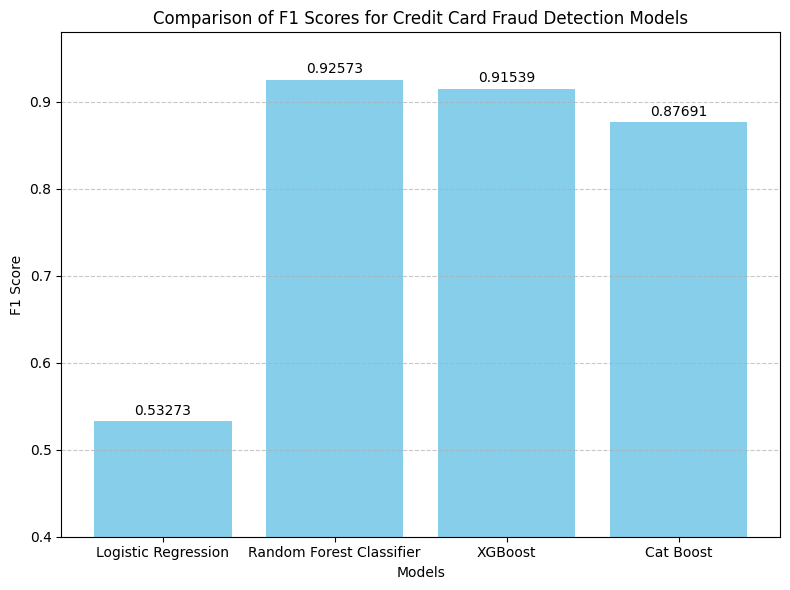
\includegraphics[scale=0.5]{figures/FinalPlot.png}
    \caption{Comparison of F1 Scores}
    \label{fig:Data Preprocessing}
\end{figure}
\clearpage


A bar plot visualization was utilized to compare the F1 scores, which indicates the Comparison of the F1 Scores of the four models. The graph showed that, in comparison to the other models, the Random Forest model performed the best and obtained the greatest F1 score.

This graphical representation made it very evident how much better the Random Forest model performed when detecting fraudulent transactions in the credit card system. These results demonstrate how important machine learning algorithms are in enhancing financial institutions' security against the constant danger of fraudulent activity. 


...





\section{Summary}







    \chapter{Discussion and Analysis}
\label{ch:evaluation}

Depending on the type of project you are doing, this chapter can be merged with ``Results'' Chapter as `` Results and Discussion'' as suggested by your supervisor. 

In the case of software development and the standalone applications, describe the significance of the obtained results/performance of the system. 



\section{A section}% please use an appropriate section title
Discussion and analysis chapter evaluates and analyses the results. It interprets the obtained results. 



\section{Significance of the findings}
In this chapter, you should also try to discuss the significance of the results and key findings, in order to enhance the reader's understanding of the investigated problem

\section{Limitations} % please discuss limitation of the project 
Discuss the key limitations and potential implications or improvements of the findings.
\section{Summary}
Write a summary of this chapter.
    \chapter{Conclusions and Future Work}
\label{ch:con}
\section{Conclusions}
In conclusion, this project has significantly improved the security of financial transactions carried out online with the development of a credit card fraud detection method. Considering the ongoing risks associated with cybercrime in the banking industry, integrating advanced machine learning algorithms offers a proactive approach to stopping fraudulent transactions. Through the use of machine learning and deep learning algorithms, the system can identify fraudulent transactions with a high degree of accuracy, which helps to reduce the amount of money that both people and financial institutions lose. The system's effectiveness and accuracy in detecting fraudulent activity in current circumstances are increased by the use of techniques like optimizing models and fine-tuning hyperparameters. The Random Forest model is particularly effective at identifying fraudulent activities, as seen by its exceptional performance. In addition to enhancing online payment security, the credit card fraud detection system developed for this project demonstrates how machine learning can efficiently tackle financial crime. Investing in technological development and research is essential to reinforcing financial institutions against emerging dangers as digital technology develops. In the future, continued research and development in this field should improve fraud detection systems even more, giving customers and businesses more protection and confidence as they negotiate the shifting landscape of online commerce.

 

\section{Future work}
There are a lot of interesting opportunities for future research and development in the field of credit card fraud detection. Using more sophisticated techniques to identify anomalous activity that may indicate fraud is an important topic to investigate. Minor indicators of fraud that conventional computer programs can overlook can be found using advanced machine learning and deep learning models and techniques like SVM, regressions, and classifiers. Applying these techniques in complex systems like detecting credit card fraud system can reduce financial loss and promote awareness amongst users and customers for secure online transactions. Using advanced technologies of AI tools, predictive modeling systems can be greatly enhanced and advanced to adapt to new challenges. To sum up, credit card fraud detection is a dynamic field that will continue to evolve due to ongoing innovation and technological investigation. Businesses and people will benefit from increased security and confidence in online transactions as a result. 
    \chapter{   Reflection}
\label{ch:reflection}
%%%%%%%%%%%%%%%%%%%%%%%%%%%%%%%
%% Please remove/replace text below
%%%%%%%%%%%%%%%%%%%%%%%%%%%%%%%
Creating a credit card fraud detection system using Python libraries has been a significant learning experience for me. While I've become more proficient in using tools like scikit-learn and pandas, the real growth came from learning how to solve complex problems and conduct effective research.

Detecting fraudulent transactions was challenging, especially with messy data that needed a lot of cleaning. Despite the difficulties, I gained valuable insights. If I were to tackle a similar project in the future, I'd prioritize data preparation to make the process smoother.

Reflecting on the project, I realized the importance of being flexible in my approach. As I delved deeper, I had to adjust my goals and methods based on new discoveries. Overall, this experience has not only enhanced my technical abilities but also deepened my understanding of problem-solving and research methodology.
    

    
    % -------------------------------------------------------------------
    % Bibliography/References  -  Harvard Style was used in this report
    % -------------------------------------------------------------------
    \bibliographystyle{agsm} % Harvard Style 
    
    \bibliography{references}  %  Patashnik, O. (1988), BibTEXing. Documentation for general BibTEX users.
    

    
    % -------------------------------------------------------------------
    % Appendices
    % -------------------------------------------------------------------
    
    \begin{appendices}
        \chapter{An Appendix Chapter (Optional)}
\label{appn:A}
% Optional chapter
Some lengthy tables, codes, raw data, length proofs, etc. which are \textbf{very important but not essential part} of the project report goes into an Appendix. An appendix is something a reader would consult if he/she needs extra information and a more comprehensive understating of the report. Also, note that you should use one appendix for one idea.

An appendix is optional. If you feel you do not need to include an appendix in your report, avoid including it. Sometime including irrelevant and unnecessary materials in the Appendices may unreasonably increase the total number of pages in your report and distract the reader.


        \chapter{An Appendix Chapter (Optional)}
\label{appn:B}

...
    \end{appendices}
    
\end{document}
